
\intro{}
\section{I numeri naturali}


\subsection{Definizione e proprietà algebriche}

\defn{L'insieme dei numeri naturali}{
L'insieme dei numeri naturali è:
\[
\mathbb{N} = \{0, 1, 2, 3, 4, \dots\}
\]

Una struttura algebrica dotata di due operazioni fondamentali: \textbf{somma} e \textbf{prodotto}.
Queste operazioni soddisfano un insieme di assiomi e proprietà che permettono
di sviluppare l'aritmetica e l'algebra su \(\mathbb{N}\).

\medskip
\textbf{Proprietà di chiusura.}
Per ogni \(x, y \in \mathbb{N}\):
\begin{itemize}
    \item \(x + y \in \mathbb{N}\) (chiusura della somma)
    \item \(x \cdot y \in \mathbb{N}\) (chiusura del prodotto)
\end{itemize}
}

\subsection{Leggi dell'algebra per la somma}

\propi{Proprietà della somma}{
    \item \textbf{Commutativa:} \(x + y = y + x\) per ogni \(x, y \in \mathbb{N}\)
    \item \textbf{Associativa:} \((x + y) + z = x + (y + z)\) per ogni \(x, y, z \in \mathbb{N}\)
    \item \textbf{Elemento neutro:} \(x + 0 = 0 + x = x\) per ogni \(x \in \mathbb{N}\)
}

\rmkb{
La proprietà commutativa significa che l'ordine in cui sommiamo due numeri non
cambia il risultato: ad esempio \(3 + 5 = 5 + 3 = 8\).
La proprietà associativa ci dice che possiamo raggruppare gli addendi in modo
diverso senza cambiare la somma: \((2+3)+4 = 2+(3+4) = 9\).
L'elemento neutro \(0\) è quello che non cambia il valore di un numero quando sommato.
}

\subsection{Leggi dell'algebra per il prodotto}

\propi{Proprietà del prodotto}{
    \item \textbf{Commutativa:} \(x \cdot y = y \cdot x\) per ogni \(x, y \in \mathbb{N}\)
    \item \textbf{Associativa:} \((x \cdot y) \cdot z = x \cdot (y \cdot z)\) per ogni \(x, y, z \in \mathbb{N}\)
    \item \textbf{Elemento neutro:} \(x \cdot 1 = 1 \cdot x = x\) per ogni \(x \in \mathbb{N}\)
}

\rmkb{
Come per la somma, nel prodotto l'ordine non conta: \(4 \times 5 = 5 \times 4 = 20\)\\[2pt]
L'elemento neutro del prodotto è \(1\): moltiplicare per \(1\) lascia invariato il numero.
}



\subsection{Leggi miste: distributività e cancellazione}

\propi{Proprietà distributiva e cancellazione}{
    \item \textbf{Distributiva:} \(x \cdot (y + z) = x \cdot y + x \cdot z\) per ogni \(x, y, z \in \mathbb{N}\)
    \item \textbf{Cancellazione della somma:} se \(x + z = y + z\), allora \(x = y\)
    \item \textbf{Cancellazione del prodotto (legge d'integrità):} 
    se \(x \cdot z = y \cdot z\) e \(z \neq 0\), allora \(x = y\)
}

\begin{esempio}
Illustriamo la proprietà distributiva e la cancellazione con esempi concreti.

\strategia{
Applichiamo la distributività “espandendo” il prodotto su una somma, 
e usiamo le leggi di cancellazione per semplificare equazioni.}

\begin{itemize}
    \item \textbf{Distributiva:}
    \[
    3 \cdot (2 + 5) = 3 \cdot 7 = 21,
    \]
    e anche
    \[
    3 \cdot 2 + 3 \cdot 5 = 6 + 15 = 21.
    \]

    \item \textbf{Cancellazione della somma:}
    Se \(x + 4 = y + 4\), allora possiamo “togliere” il \(4\) da entrambi i lati
    e concludere che \(x = y\).

    \item \textbf{Cancellazione del prodotto:}
    Se \(3x = 3y\) con \(3 \neq 0\), possiamo “dividere per 3” e concludere che \(x = y\).
\end{itemize}
\end{esempio}

\section{Ordinamento sui numeri naturali}

\defn{Ordinamento e tricotomia}{
L'ordinamento sui numeri naturali si definisce come:
\[
x \leq y \quad \text{se e solo se} \quad \exists z \in \mathbb{N} : x + z = y.
\]

L'ordinamento stretto è:
\[
x < y \quad \text{se e solo se} \quad x \leq y \text{ e } x \neq y.
\]

Una proprietà fondamentale è la \textbf{legge di tricotomia}: dati due numeri naturali \(x\) e \(y\),
vale esattamente una delle seguenti tre condizioni:
\begin{itemize}
    \item \(x < y\), oppure
    \item \(y < x\), oppure
    \item \(x = y\).
\end{itemize}
}

\rmkb{
La tricotomia ci assicura che fra due numeri naturali c'è sempre una relazione d'ordine:
uno è minore dell'altro, oppure sono uguali. Non ci sono casi ambigui.
}

\thm{L'ordinamento è un ordinamento totale}{
L'ordinamento \(\leq\) su \(\mathbb{N}\) soddisfa:
\begin{itemize}
    \item \textbf{Riflessiva:} \(x \leq x\) per ogni \(x \in \mathbb{N}\)
    \item \textbf{Antisimmetrica:} se \(x \leq y\) e \(y \leq x\), allora \(x = y\)
    \item \textbf{Transitiva:} se \(x \leq y\) e \(y \leq z\), allora \(x \leq z\)
\end{itemize}
Quindi \(\leq\) è un ordinamento totale su \(\mathbb{N}\).
}

\begin{esempio}
Verifichiamo che l'ordinamento \(\leq\) su \(\mathbb{N}\) è riflessivo, antisimmetrico e transitivo.

\strategia{
Usiamo la definizione \(x \leq y \Leftrightarrow \exists z \in \mathbb{N} : x + z = y\) e le leggi dell’algebra sui naturali.
}
\textbf{Riflessiva.}
Per ogni \(x \in \mathbb{N}\) vale \(x \leq x\).
Infatti esiste \(z = 0 \in \mathbb{N}\) tale che \(x + 0 = x\).

\medskip
\textbf{Antisimmmetrica.}
Per ogni \(x, y \in \mathbb{N}\), se \(x \leq y\) e \(y \leq x\) allora \(x = y\).
Dalla definizione di \(\leq\), se \(x \leq y\) e \(y \leq x\) esistono \(k, r \in \mathbb{N}\) tali che
\[
x + k = y \quad \text{e} \quad y + r = x.
\]
Quindi
\[
x + (k + r) = (x + k) + r = y + r = x.
\]
Poiché \(x = x + 0\), dalla proprietà di cancellazione della somma otteniamo
\[
x + (k + r) = x + 0 \;\Rightarrow\; k + r = 0.
\]
Ma l’unico modo di avere \(k + r = 0\) con \(k, r \in \mathbb{N}\) è \(k = r = 0\).
Allora \(x = x + 0 = x + k = y\), cioè \(x = y\).

\medskip
\textbf{Transitiva.}
Per ogni \(x, y, z \in \mathbb{N}\), se \(x \leq y\) e \(y \leq z\) allora \(x \leq z\).
Dalla definizione di \(\leq\), esistono \(k, r \in \mathbb{N}\) tali che
\[
x + k = y \quad \text{e} \quad y + r = z.
\]
Allora
\[
x + (k + r) = (x + k) + r = y + r = z,
\]
quindi esiste \(k + r \in \mathbb{N}\) con \(x + (k + r) = z\), cioè \(x \leq z\).
\end{esempio}

\section{Multipli e divisibilità}

\defn{Multipli e divisibilità}{
Siano \(m, n \in \mathbb{N}\). Diciamo che \(m\) è un \textbf{multiplo} di \(n\)
se esiste un numero naturale \(a \in \mathbb{N}\) tale che:
\[
m = a \cdot n.
\]

In questo caso, diciamo anche che \(n\) \textit{divide} \(m\), e scriviamo \(n \mid m\).
}

\rmkb{
Esempi: \(12\) è un multiplo di \(3\) perché \(12 = 4 \cdot 3\), quindi \(3 \mid 12\).
Analogamente, \(15\) è multiplo di \(5\) (\(15 = 3 \cdot 5\)), quindi \(5 \mid 15\).
}

\thm{Proprietà dei multipli}{
Se \(a\) e \(b\) sono multipli di \(n\), allora \(xa + yb\) è un multiplo di \(n\)
per ogni \(x, y \in \mathbb{N}\).
}

\begin{thmpf}
Poiché \(a\) e \(b\) sono multipli di \(n\), esistono \(r, s \in \mathbb{N}\) tali che:
\[
a = r \cdot n, \quad b = s \cdot n.
\]

Allora:
\[
xa + yb = x(rn) + y(sn) = (xr + ys)\cdot n.
\]

Poiché \(xr + ys \in \mathbb{N}\), segue che \(xa + yb\) è un multiplo di \(n\).
\end{thmpf}

\begin{esempio}
Applichiamo il teorema con numeri concreti.

\strategia{
Verifichiamo che combinazioni lineari di multipli di \(n\) restano multipli di \(n\).}

\begin{itemize}
    \item Sia \(n=3\). Allora \(6\) è multiplo di \(3\) (\(6=2\cdot 3\)) e \(9\) è multiplo di \(3\) (\(9=3\cdot 3\)).
    \item Prendiamo \(x=2\) e \(y=3\):
    \[
    2\cdot 6 + 3\cdot 9 = 12 + 27 = 39.
    \]
    \item Controlliamo: \(39 = 13\cdot 3\), quindi \(3 \mid 39\), come previsto.
\end{itemize}
\end{esempio}

\section{Proprietà di buon ordinamento}

\defn{Insieme ben ordinato}{
Un insieme \(A\) dotato di una relazione d'ordine \(\leq\) si dice \textbf{ben ordinato}
se ogni sottoinsieme non vuoto di \(A\) ha un elemento minimo.
}

\thm{I numeri naturali sono ben ordinati}{
L'insieme \(\mathbb{N}\), con la relazione d'ordine \(\leq\), è ben ordinato.
In particolare:
\begin{itemize}
    \item \(0\) è il minimo elemento di \(\mathbb{N}\): \(0 \leq x\) per ogni \(x \in \mathbb{N}\);
    \item ogni sottoinsieme non vuoto di \(\mathbb{N}\) ha un elemento minimo.
\end{itemize}
}

\rmkb{
La proprietà di buon ordinamento di \(\mathbb{N}\) è alla base del principio di induzione.
È ciò che rende \(\mathbb{N}\) “speciale” rispetto ad altri insiemi come \(\mathbb{Z}\) o \(\mathbb{Q}\),
dove non sempre esiste un minimo per ogni sottoinsieme non vuoto.
}









































\section{Introduzione al principio di induzione}

% \defn{Principio di induzione}{
% Il principio di induzione è una tecnica di dimostrazione che permette di
% mostrare che una proprietà \(P(n)\) vale per \emph{tutti} i numeri naturali.

% Per provare che \(P(n)\) è vera per ogni \(n\in\mathbb{N}\) basta:

% \begin{enumerate}
%     \item \textbf{Caso base}: dimostrare che la proprietà è vera per il primo
%     valore considerato (ad esempio \(n=0\) in \(\mathbb{N}\), oppure \(n=1\) in \(\mathbb{N}^+\)).

%     \item \textbf{Passo induttivo}: assumere che la proprietà sia vera per un
%     numero arbitrario \(k\) (ipotesi induttiva: \(P(k)\) è vera) e, sotto
%     questa ipotesi, dimostrare che è vera anche per \(k+1\):
%     \[
%         P(k) \implies P(k+1).
%     \]
% \end{enumerate}

% Se entrambi i passi sono corretti, allora \(P(n)\) è vera per ogni \(n\)
% naturale.
% }
\defn{Principio di induzione}{
Sia \(P(x)\) una proprietà dei numeri naturali.
\medskip

\noindent 

Il principio di induzione dice che,  per dimostrare  che \(P(x)\) è vera per ogni numero naturale \(x\), è sufficiente dimostrare: 
\begin{itemize}
    \item \textbf{Caso base } \(P(0)\) è vera (cioè la proprietà vale per il numero \(0\)).
    \item \textbf{Passo induttivo}: per ogni \(n \geq 0\),
    \[
        P(n) \implies P(n+1),
    \]
    cioè se \(P(n)\) è vera, allora \(P(n+1)\) è vera.
\end{itemize}
In altri termini:
\[
P(0) \,\wedge\, \forall x \bigl(P(x) \Rightarrow P(x+1)\bigr) \;\Rightarrow\; \forall x\, P(x).
\]

In altre parole, per provare che \(P(x)\) è vera per ogni numero naturale \(x\), è sufficiente:
\begin{itemize}
    \item verificare il \textbf{caso base} \(P(0)\);
    \item assumere \(P(n)\) vera per un generico \(n \geq 0\)
          (\textbf{ipotesi induttiva}) e, usando questa ipotesi,
          dimostrare \(P(n+1)\) (\textbf{passo induttivo}).
\end{itemize}
}

\begin{esempio}
    Dimostrare che la somma dei primi \(n\) numeri naturali è uguale a \(\dfrac{n(n+1)}{2}\), per ogni numero intero \(n \geq 1\):
    \[
    S(n)= 1+2+3\ldots + n = \dfrac{n(n+1)}{2}
    \]
    \strategia{
    Useremo il principio di induzione: Verifichiamo la formula per \(n=1\), poi supponiamo che \(n= k\) e infine la dimostriamo per \(n=k+1\).
    }

    \begin{itemize}
        \item \textbf{Caso base} \(n=1\).
        \[
        S(1)=, \quad \dfrac{1(1+1)}{2}= \dfrac{2}{2}=1
        \]
    Quindi la formula è verificata per \(n=1\)
    \item \textbf{Ipotesi induttiva}: Supponiamo che per un certo \(k \geq 1 \) valga:
    \[
    S(k)= 1+2+3+\ldots k = \dfrac{k(k+1)}{2}
    \]
    \item  \textbf{Passo induttivo}
    Vogliamo mostrare:
     \[
    S(k+1) = 1 + 2 + \ldots + k + (k+1) = \frac{(k+1)(k+2)}{2}.
    \]
    Per definizione:
    \[
    S(k+1) = S(k) + (k+1).
    \]
    Sostituendo l’ipotesi induttiva:
    \[
    S(k+1) = \frac{k(k+1)}{2} + (k+1).
    \]
    Mettiamo \(k+1\) in evidenza:
    \[
    S(k+1) = \frac{k(k+1) + 2(k+1)}{2}
           = \frac{(k+1)(k+2)}{2}.
    \]
    Quindi la formula è vera anche per \(k+1\).
    \end{itemize}
    Per il principio di induzione, la formula vale per ogni \(n \geq 1\)
\end{esempio}







\begin{esempio}
    Dimostrare per induzione che per ogni \(n \in \mathbb{N}\) esiste \(m \in \mathbb{Z}\) tale che
\[
n^3 + 5n = 6m,
\]
cioè \(n^3+5n\) è sempre divisibile per \(6\).
\strategia{Mostriamo che la proprietà vale per \(n=0\) , poi assumiamo che valga per un generico \(n\) verifichiamo che allora vale anche per \(n+1\) }
\begin{itemize}
    \item \textbf{Caso base} (\(n=0\)):
    \[
    0^3 + 5\cdot 0 = 0,
    \]
    che è divisibile per \(6\). Quindi la proprietà vale per \(n=0\).

    \item \textbf{Ipotesi induttiva}:
    supponiamo che esista \(m \in \mathbb{Z}\) tale che
    \[
    n^3 + 5n = 6m
    \]
    per un certo \(n \in \mathbb{N}\).

    \item \textbf{Passo induttivo}:
    verifichiamo la proprietà per \(n+1\):
    \[
    (n+1)^3 + 5(n+1)
    = n^3 + 3n^2 + 3n + 1 + 5n + 5
    = n^3 + 5n + 3n^2 + 3n + 6.
    \]
    Sostituendo l’ipotesi induttiva \(n^3 + 5n = 6m\), otteniamo:
    \[
    (n+1)^3 + 5(n+1) = 6m + 3n^2 + 3n + 6.
    \]
    Mettiamo in evidenza:
    \[
    6m + 3n^2 + 3n + 6
    = 6m + 3n(n+1) + 6.
    \]
    Osserviamo che \(n(n+1)\) è sempre pari (prodotto di due interi consecutivi),
    quindi esiste \(r \in \mathbb{Z}\) tale che \(n(n+1) = 2r\). Allora:
    \[
    6m + 3n(n+1) + 6
    = 6m + 3\cdot 2r + 6
    = 6(m + r + 1).
    \]
    Dunque \((n+1)^3 + 5(n+1)\) è di nuovo multiplo di \(6\).
\end{itemize}

Per il principio di induzione, \(n^3 + 5n\) è divisibile per \(6\) per ogni \(n \in \mathbb{N}\).
\end{esempio}

\section{Principio di induzione con base k}
\defn{Principio di induzione con base \(k\)}{
Sia \(P(x)\) una proprietà sui numeri naturali e sia \( k \in \NN \).

Per dimostrare che \(P(x)\) è vera per ogni numero naturale \(x \ge k\) è sufficiente:

\begin{enumerate}
    \item \textbf{Caso base}: dimostrare che la proprietà è vera per \(x = k\),
    cioè \(P(k)\) è vera.

    \item \textbf{Passo induttivo}: per ogni \(x \ge k\), assumere che \(P(x)\) sia vera
    (ipotesi induttiva) e, sotto questa ipotesi, dimostrare che è vera anche per \(x+1\):
    \[
        x \ge k \ \wedge\ P(x) \ \Longrightarrow\ P(x+1).
    \]
\end{enumerate}

In altri termini:
\[
P(k) \ \wedge\ \forall x\bigl(x \ge k \wedge P(x) \Rightarrow P(x+1)\bigr)
\ \Rightarrow\ \forall x\bigl(x \ge k \Rightarrow P(x)\bigr).
\]
}










\begin{esempio}
\textbf{La torre di Hanoi}

La leggenda racconta che esiste un tempio indu\'`  in cui si trova una torre composta
da \(64\) dischi d’oro, tutti di grandezza diversa, bucati al centro e infilati su un piolo
di diamante. Il disco più grande giace sul fondo, e i dischi successivi sono via via
più piccoli fino al più piccolo in cima. Nel tempio ci sono anche altri due pioli di
diamante, quindi in totale tre pioli.
\begin{center}
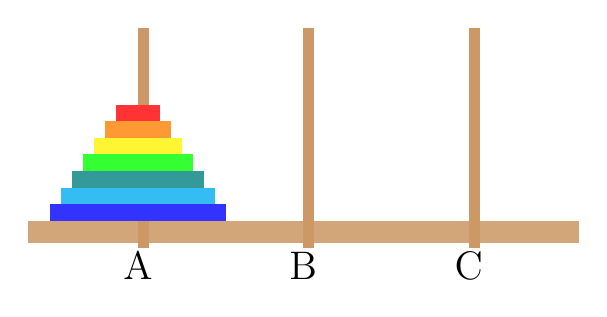
\begin{tikzpicture}[scale=0.7]

  
  \fill[brown!70] (-5,0) rectangle (5,0.4);

  \foreach \x in {-3,0,3} {
    \fill[brown!80] (\x,-0.1) rectangle ++(0.2,4);
  }

  \def\h{0.3}

  \fill[blue!80!white]   (-3-1.6, 0.4+0*\h) rectangle ++(2*1.6,\h);
  \fill[cyan!80!white]   (-3-1.4, 0.4+1*\h) rectangle ++(2*1.4,\h);
  \fill[teal!80!white]   (-3-1.2, 0.4+2*\h) rectangle ++(2*1.2,\h);
  \fill[green!80!white]  (-3-1.0, 0.4+3*\h) rectangle ++(2*1.0,\h);
  \fill[yellow!80!white] (-3-0.8, 0.4+4*\h) rectangle ++(2*0.8,\h);
  \fill[orange!80!white] (-3-0.6, 0.4+5*\h) rectangle ++(2*0.6,\h);
  \fill[red!80!white]    (-3-0.4, 0.4+6*\h) rectangle ++(2*0.4,\h);

  \node[below] at (-3,0) {\Large A};
  \node[below] at (0,0)  {\Large B};
  \node[below] at (3,0)  {\Large C};

\end{tikzpicture}
\end{center}

\medskip


\begin{center}
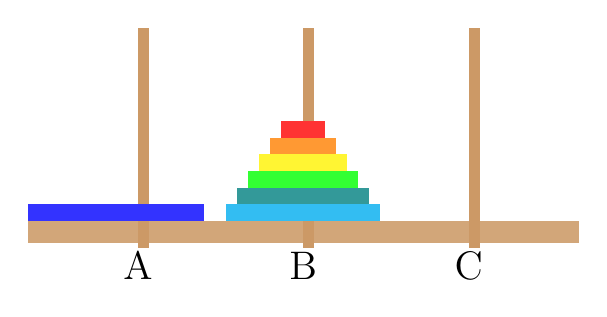
\begin{tikzpicture}[scale=0.7]
  \fill[brown!70] (-5,0) rectangle (5,0.4);
  \foreach \x in {-3,0,3} {
    \fill[brown!80] (\x,-0.1) rectangle ++(0.2,4);
  }
  \def\h{0.3}
  % dischi: base su A, altri su B
  \fill[blue!80!white]   (-3.4-1.6, 0.4+0*\h) rectangle ++(2*1.6,\h);
 \fill[cyan!80!white]    (0-1.4, 0.4+0*\h) rectangle ++(2*1.4,\h);
  \fill[teal!80!white]   (0-1.2, 0.4+1*\h) rectangle ++(2*1.2,\h);
  \fill[green!80!white]  (0-1.0, 0.4+2*\h) rectangle ++(2*1.0,\h);
  \fill[yellow!80!white] (0-0.8, 0.4+3*\h) rectangle ++(2*0.8,\h);
  \fill[orange!80!white] (0-0.6, 0.4+4*\h) rectangle ++(2*0.6,\h);
  \fill[red!80!white]    (0-0.4, 0.4+5*\h) rectangle ++(2*0.4,\h);

  \node[below] at (-3,0) {\Large A};
  \node[below] at (0,0)  {\Large B};
  \node[below] at (3,0)  {\Large C};
\end{tikzpicture}
\hspace{1cm}
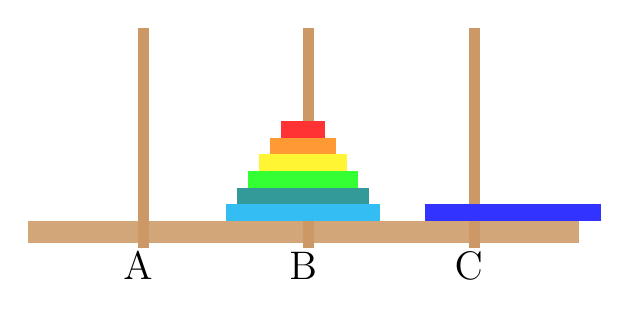
\begin{tikzpicture}[scale=0.7]
  \fill[brown!70] (-5,0) rectangle (5,0.4);
  \foreach \x in {-3,0,3} {
    \fill[brown!80] (\x,-0.1) rectangle ++(0.2,4);
  }
  \def\h{0.3}
  % dischi: base su C, altri su B
  \fill[blue!80!white]   (3.2-1., 0.4+0*\h)  rectangle ++(2*1.6,\h);
 \fill[cyan!80!white]    (0-1.4, 0.4+0*\h) rectangle ++(2*1.4,\h);
  \fill[teal!80!white]   (0-1.2, 0.4+1*\h) rectangle ++(2*1.2,\h);
  \fill[green!80!white]  (0-1.0, 0.4+2*\h) rectangle ++(2*1.0,\h);
  \fill[yellow!80!white] (0-0.8, 0.4+3*\h) rectangle ++(2*0.8,\h);
  \fill[orange!80!white] (0-0.6, 0.4+4*\h) rectangle ++(2*0.6,\h);
  \fill[red!80!white]    (0-0.4, 0.4+5*\h) rectangle ++(2*0.4,\h);

  \node[below] at (-3,0) {\Large A};
  \node[below] at (0,0)  {\Large B};
  \node[below] at (3,0)  {\Large C};
\end{tikzpicture}
\end{center}

\medskip 

\begin{center}
    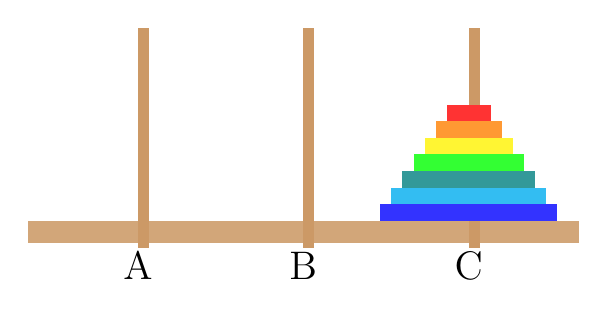
\begin{tikzpicture}[scale=0.7]
  \fill[brown!70] (-5,0) rectangle (5,0.4);
  \foreach \x in {-3,0,3} {
    \fill[brown!80] (\x,-0.1) rectangle ++(0.2,4);
  }
  \def\h{0.3}
  % dischi: base su C, altri su B
  \fill[blue!80!white]   (3-1.6, 0.4+0*\h)  rectangle ++(2*1.6,\h);
  \fill[cyan!80!white]   (3-1.4, 0.4+1*\h) rectangle ++(2*1.4,\h);
  \fill[teal!80!white]   (3-1.2, 0.4+2*\h) rectangle ++(2*1.2,\h);
  \fill[green!80!white]  (3-1.0, 0.4+3*\h) rectangle ++(2*1.0,\h);
  \fill[yellow!80!white] (3-0.8, 0.4+4*\h) rectangle ++(2*0.8,\h);
  \fill[orange!80!white] (3-0.6, 0.4+5*\h) rectangle ++(2*0.6,\h);
  \fill[red!80!white]    (3-0.4, 0.4+6*\h) rectangle ++(2*0.4,\h);

  \node[below] at (-3,0) {\Large A};
  \node[below] at (0,0)  {\Large B};
  \node[below] at (3,0)  {\Large C};
\end{tikzpicture}
\end{center}






















Alcuni monaci buddisti hanno il compito di spostare \emph{l’intera piramide} da un piolo
a un altro, muovendo un solo disco alla volta e usando il terzo piolo come appoggio.
Devono rispettare una regola fondamentale:
\begin{itemize}
    \item non è mai permesso mettere un disco su un disco più piccolo.
\end{itemize}
La leggenda dice che, quando i monaci avranno spostato tutta la torre, il mondo finirà.

\strategia{
Vogliamo capire \emph{quante mosse} servono almeno per spostare una torre di \(n\) dischi.
Chiameremo \(H(n)\) il numero minimo di mosse per spostare una piramide di \(n\) dischi
da un piolo a un altro, rispettando le regole. Dimostreremo per induzione che
\[
H(n) = 2^n - 1.
\]
Questo ci permetterà anche di stimare quanto tempo impiegherebbero i monaci con \(64\) dischi.
}
\medskip
\textbf{Come funziona la strategia ottimale}

Per spostare una torre di \(n+1\) dischi dal piolo \(A\) al piolo \(C\) usando \(B\) come appoggio,
non possiamo muovere subito il disco più grande (quello alla base), perché sopra di lui
ci sono \(n\) dischi più piccoli. La strategia naturale (e in realtà ottimale) è:

\begin{enumerate}
    \item Spostare i primi \(n\) dischi (i più piccoli) da \(A\) a \(B\), usando \(C\) come piolo intermedio.
    \item Spostare il disco più grande (alla base) da \(A\) a \(C\).
    \item Spostare di nuovo i \(n\) dischi più piccoli da \(B\) a \(C\), usando \(A\) come piolo intermedio.
\end{enumerate}

In ognuna delle fasi 1) e 3) stiamo risolvendo lo \emph{stesso} problema, ma con \(n\) dischi
invece che \(n+1\).

\medskip
\textbf{Definizione formale.}
Per ogni \(n \in \mathbb{N}\), definiamo:
\[
H(n) = \text{numero minimo di mosse per spostare una torre di \(n\) dischi da un piolo a un altro.}
\]

\medskip
\textbf{Dimostrazione per induzione che \(H(n)=2^n-1\).}

\textit{Caso base.} Sia \(n = 1\). Se c’è un solo disco, basta una mossa per
spostarlo da un piolo a un altro, quindi:
\[
H(1) = 1 = 2^1 - 1.
\]
La formula è vera per \(n=1\).

\medskip
\textit{Ipotesi induttiva.} Sia \(n \geq 1\). Supponiamo che la formula sia vera
per \(n\), cioè:
\[
H(n) = 2^n - 1.
\]

\medskip
\textit{Passo induttivo.} Vogliamo calcolare \(H(n+1)\).

Per spostare una torre di \(n+1\) dischi da \(A\) a \(C\) usando \(B\) come appoggio
dobbiamo procedere così:

\begin{enumerate}
    \item Spostare i \(n\) dischi più piccoli da \(A\) a \(B\): servono \(H(n)\) mosse.
    \item Spostare il disco più grande da \(A\) a \(C\): serve 1 mossa.
    \item Spostare i \(n\) dischi più piccoli da \(B\) a \(C\): servono di nuovo \(H(n)\) mosse.
\end{enumerate}

Quindi il numero totale di mosse è:
\[
H(n+1) = H(n) + 1 + H(n) = 2H(n) + 1.
\]
Usando l’ipotesi induttiva \(H(n) = 2^n - 1\) otteniamo:
\[
H(n+1) = 2(2^n - 1) + 1
       = 2^{n+1} - 2 + 1
       = 2^{n+1} - 1.
\]
La formula vale quindi anche per \(n+1\).

Per il principio di induzione, per ogni \(n \in \mathbb{N}\) si ha:
\[
H(n) = 2^n - 1.
\]

\medskip
\textbf{Cosa significa per i 64 dischi della leggenda?}

Per \(n = 64\):
\[
H(64) = 2^{64} - 1,
\]
che è un numero enorme di mosse. Anche spostando un disco al secondo,
i monaci impiegherebbero centinaia di miliardi di anni per completare il lavoro.
Perfino lavorando a \(1000\) mosse al secondo, servirebbero comunque centinaia di milioni di anni.
Quindi, almeno secondo questo modello, la fine del mondo non è così vicina.
\end{esempio}


\section{Forma forte del principio di induzione}
\defn{Forma forte del principio di induzione}{
Sia $P(x)$ una proprietà sui numeri naturali. Per dimostrare che $P(x)$ è vera per ogni numero naturale $x \in \mathbb{N}$, è sufficiente dimostrare che:

\begin{enumerate}
    \item $P(0)$ è vera (caso base esteso).
    \item $\forall n \geq 0$, se $P(0) \wedge P(1) \wedge \cdots \wedge P(n)$ sono tutte vere, allora $P(n+1)$ è vera (passo induttivo forte).
\end{enumerate}
In altri termini:
\[
    P(0) \land \forall x (P(0) \land P(1) \land \ldots \land P(x) \Rightarrow P(x+1) ) \Rightarrow \forall x (P(x)) 
\]

 A differenza del principio di induzione classica (che assume solo $P(n) \implies P(n+1)$), la forma forte permette di usare \emph{tutti} i casi precedenti $P(0),\dots,P(n)$ per dimostrare $P(n+1)$.
}


\subsection{Forma forte del principio di induzione con base k}
\defn{Forma forte del principio di induzione con base $k$}{
Sia \(P(x)\) una proprietà sui numeri naturali. Per dimostrare che \(P(x)\) è vera per ogni \(x \geq k\), con \(k \in \NN\), è sufficiente dimostrare:
\begin{itemize}
    \item \(P(k)\)è vera (caso base generalizzato a \(k\))
    \item \(P(k) \land \ldots \land P(n) \Rightarrow P(n+1) \ \forall n \geq k\) sono tutte vere, allora $P(n+1)$ è vera (passo induttivo forte).
\end{itemize}
In altri termini:
\[
P(k)\land \forall x (P(k) \land \ldots \land P(x) \Rightarrow P(x+1) ) \Rightarrow \forall x (P(x))
\]

Questa generalizzazione sposta il caso base da $0$ a un arbitrario $k$, mantenendo la forza dell'ipotesi induttiva che usa \emph{tutti} i casi da $k$ a $n$. È utile quando la proprietà parte da un valore specifico, come $P(n)$ per $n \geq 2$ in teoremi su numeri pari/dispari.
}





\section{I numeri naturali }


\defn{I numeri naturali definizione induttiva}{
Il principio di induzione si applica facilmente ai numeri naturali perché essi sono definiti “induttivamente” a partire dal numero \(0\) e applicando l'operazione di successore \((+1)\).

I numeri naturali sono definiti induttivamente nel seguente modo:
\begin{itemize}
    \item \(0\) è un numero naturale;
    \item se \(n\) è un numero naturale allora anche il suo successore \(n + 1\) è un numero naturale;
    \item nient’altro è un numero naturale.
\end{itemize}

Il principio di induzione per i numeri naturali è il seguente:
\[
P(0) \forall x ( P(x) \Rightarrow P(x+1) ) \Rightarrow \forall x P(x)
\]
}



\section{Stringhe ed espressioni}


\subsection{Stringhe}




\defn{Le stringhe (definizione induttiva)}{
    Le stringhe (o parole) su un alfabeto \( A \) sono sequenze finite di elementi di \( A \). 
    
    Le stringhe sull'alfabeto \( \{a, b\} \) sono definite induttivamente nel seguente modo:
    \begin{itemize}
        \item \( \varepsilon \) (la sequenza vuota) è una stringa;
        \item se \( \alpha \) è una stringa, allora la concatenazione \( \alpha a \) della stringa \( \alpha \) e del carattere \( a \) è una stringa;
        \item se \( \alpha \) è una stringa, allora la concatenazione \( \alpha b \) della stringa \( \alpha \) e del carattere \( b \) è una stringa;
        \item nient'altro è una stringa.
    \end{itemize}

     Questa definizione ci dice che l'insieme delle stringhe è il più piccolo insieme che contiene la sequenza vuota ed è chiuso rispetto all'operazione di aggiunta di un carattere alla destra della stringa corrente. Ogni stringa non vuota è quindi costruita a partire da \( \varepsilon \) in un numero finito di passi.
}











\thmr{Principio di induzione strutturale per le stringhe}{ind_stringhe}{
    Sia \( P \) una proprietà sulle stringhe e siano \( \alpha \) e \( \beta \) variabili che assumono valori sull'insieme delle stringhe. Il principio di induzione per il tipo di dato stringa è il seguente:
    \[
    P(\varepsilon) \land \forall \alpha \big( P(\alpha) \implies P(\alpha a) \land P(\alpha b) \big) \implies \forall \alpha P(\alpha)
    \]

    Per dimostrare che una proprietà vale per ogni possibile stringa, non è necessario testarle tutte (che sono infinite). È sufficiente verificare che valga per la stringa "base" (\( \varepsilon \)) e che, assumendola vera per una stringa \( \alpha \), la proprietà si conservi quando costruiamo stringhe più lunghe aggiungendo \( a \) o \( b \).
}




\begin{esempio}
    
    Dimostrare, per induzione strutturale, che la lunghezza della stringa \( \alpha\alpha \) è un numero pari, per ogni stringa \( \alpha \).


\strategia{
    Utilizzeremo il principio di induzione strutturale appena definito. 
    Dobbiamo verificare la proprietà per la stringa vuota (caso base) e poi mostrare che, se la proprietà vale per una generica stringa \( \alpha \), essa continua a valere anche per le stringhe estese \( \alpha a \) e \( \alpha b \). L'idea chiave è sfruttare le proprietà della lunghezza rispetto alla concatenazione.
}

    Indichiamo con \( \ell(\alpha) \) la lunghezza di una stringa \( \alpha \).
    
    \textbf{Caso base:} Sia \( \alpha = \epsilon \). \\
    Poiché \( \epsilon\epsilon = \epsilon \), abbiamo che:
    \[ \ell(\epsilon\epsilon) = \ell(\epsilon) = 0 \]
    Poiché 0 è un numero pari, il caso base è verificato.

    \textbf{Passo induttivo:} Sia \( \alpha \) una stringa generica. \\
    Supponiamo la seguente \textbf{ipotesi induttiva}: \( \ell(\alpha\alpha) \) è pari.

   Dobbiamo dimostrare la tesi per la stringa \( \alpha a \) (il ragionamento per \( \alpha b \) è analogo).
    Consideriamo la stringa composta \( (\alpha a)(\alpha a) \), che possiamo scrivere come \( \alpha a \alpha a \).
    Se permutiamo i caratteri presenti in una stringa la sua lunghezza non cambia (la lunghezza è additiva). Quindi:
    \[
    \ell(\alpha a \alpha a) = \ell(\alpha \alpha a a) = \ell(\alpha \alpha) + \ell(a a) = \ell(\alpha \alpha) + 2
    \]
    Per ipotesi induttiva, sappiamo che \( \ell(\alpha\alpha) \) è pari. Poiché la somma di due numeri pari è pari (\( \text{pari} + 2 = \text{pari} \)), ne segue che anche \( \ell(\alpha a \alpha a) \) è pari.
    
    Un ragionamento identico vale per la stringa \( \alpha b \).
    Ne segue, per il principio di induzione, che ogni stringa \( \alpha\alpha \) ha lunghezza pari.

\end{esempio}
  \rmkb{
    Notiamo come in questo esercizio la natura specifica dei caratteri 'a' o 'b' non sia rilevante ai fini della dimostrazione, ma solo il fatto che aggiungono 1 alla lunghezza totale. L'induzione strutturale ci permette di generalizzare questo comportamento costruttivo.
  }






















\defn{ Espressioni aritmetiche (definizione induttiva)}{
    Siano \( a, 0, 1, [, ], +, * \) dei caratteri. L'insieme EXP delle espressioni aritmetiche è definito induttivamente come segue:
    \begin{itemize}
        \item \( a, 0, 1 \) sono espressioni;
        \item se \( E_1 \) e \( E_2 \) sono espressioni allora \( [E_1 + E_2] \) e \( [E_1 * E_2] \) sono espressioni;
        \item nient'altro è una espressione.
    \end{itemize}
    Per esempio, le stringhe \( [a + 1] \) e \( [0 + [a * 0]] \) sono espressioni, mentre le stringhe \( [a + 1[ \) e \( [ ] \) non sono espressioni.
    
    Questa definizione stabilisce una sintassi rigorosa. Le espressioni "atomiche" (base) non hanno parentesi. Ogni volta che si combinano due espressioni con un operatore, è \textit{obbligatorio} racchiudere il risultato tra parentesi quadre. Questo elimina ogni ambiguità sull'ordine delle operazioni.
}







\thmr{Principio di induzione strutturale per le espressioni}{ind_exp}{
    Sia \( P \) una proprietà sulle espressioni aritmetiche. Siano \( x \) e \( y \) variabili che assumono valori sull'insieme delle espressioni aritmetiche. Il principio di induzione per il tipo di dato espressione è come segue:
    \[
    P(a) \land P(0) \land P(1) \land \forall x,y \big( P(x) \land P(y) \implies P([x + y]) \land P([x * y]) \big) \implies \forall x P(x)
    \]

     La struttura di questo principio riflette la definizione ricorsiva. Abbiamo tre casi base da verificare singolarmente. Il passo induttivo richiede di assumere la proprietà vera per due sotto-espressioni qualsiasi \( x \) e \( y \), per poi dimostrare che la proprietà si mantiene quando queste vengono combinate tramite somma o prodotto.
}




















\begin{esempio}
    Dimostrare, per induzione strutturale, che ogni espressione aritmetica ha un numero pari di parentesi.
    \strategia{
    Procederemo contando le parentesi presenti nei casi base (atomi) e osservando quante parentesi vengono aggiunte durante il passo di costruzione ricorsiva. Poiché le regole di costruzione aggiungono parentesi sempre a coppie (aperta e chiusa), ci aspettiamo che la parità si conservi.
}

Indichiamo con \( p(E) \) il numero di parentesi dell'espressione \( E \).
    
    \textbf{Caso base:} Le espressioni \( a \), \( 0 \) e \( 1 \) sono atomiche e non contengono parentesi.
    \[
    p(a) = p(0) = p(1) = 0
    \]
    Poiché 0 è un numero pari, la proprietà è verificata per i casi base.

    \textbf{Passo induttivo:} Siano \( E_1 \) ed \( E_2 \) due espressioni generiche.
    Supponiamo che \( E_1 \) ed \( E_2 \) abbiano un numero pari di parentesi.
    \textbf{Ipotesi induttiva:} \( p(E_1) \) e \( p(E_2) \) sono numeri pari.
    
    Consideriamo l'espressione composta \( [E_1 + E_2] \). Il numero totale di parentesi è dato dalle parentesi già presenti in \( E_1 \), più quelle in \( E_2 \), più la coppia di parentesi quadre esterna che racchiude la somma. Si ha:
    \[
    p([E_1 + E_2]) = p(E_1) + p(E_2) + 2
    \]
    Analizziamo la parità:
    \begin{itemize}
        \item \( p(E_1) \) è pari per ipotesi induttiva;
        \item \( p(E_2) \) è pari per ipotesi induttiva;
        \item 2 è un numero pari.
    \end{itemize}
    Poiché la somma di numeri pari è sempre pari, \( p([E_1 + E_2]) \) è un numero pari.
    
    Un ragionamento del tutto simile vale per l'espressione \( [E_1 * E_2] \).
\end{esempio}





\rmkb{
    Questo risultato è una conseguenza diretta della sintassi rigida definita induttivamente. Se la definizione permettesse di omettere le parentesi esterne (come in aritmetica standard), questa proprietà non sarebbe più necessariamente vera o richiederebbe una dimostrazione molto più complessa sulla grammatica del linguaggio.
}







\section{ Ricorsione}









\defn{Funzioni ricorsive }{
Se $A$ è un insieme definito per induzione allora possiamo definire ricorsivamente funzioni con dominio $A$.

Abbiamo visto che i numeri naturali sono definiti "induttivamente" a partire dal numero $0$ e applicando l'operazione di successore $(+1)$. Questo permette di definire funzioni come somma e prodotto in modo ricorsivo, seguendo esattamente la struttura induttiva di $\mathbb{N}$.
}


\begin{esempio}
\textbf{Funzione potenza di 2} $f(n)= 2^n$

La funzione è definita come segue:
\[
f: \mathbb{N} \to \mathbb{N}, \quad f(n)= 
\begin{cases}
    1  & \text{se } n = 0 \\
    2 \cdot f(n-1)  & \text{se } n >0
\end{cases}
\]

O equivalentemente:
\[
2^n = 2^0 \cdot 2^1 \cdot 2^2 \ldots \cdot 2^n
\]

\begin{tcolorbox}[
    colback=backcolour, 
    colframe=framegray, 
    boxrule=0.5pt, 
    sharp corners,
    left=5mm, right=5mm, 
    top=5mm, bottom=5mm,
    width=\linewidth
]
\begin{lstlisting}
int pow(int n){
    if(n == 0 ) // caso base
        return 1;
    else 
        return 2 * pow(n-1); // passo ricorsivo
}
\end{lstlisting}
\end{tcolorbox}

\strategia{
Dimostreremo per induzione su $n$ che la funzione $\text{pow}(n)$ termina sempre e restituisce correttamente $2^n$ per ogni $n \in \mathbb{N}$. Verificheremo il caso base $n=0$ e mostreremo che, assumendo la correttezza per $n-1$, essa vale anche per $n$.
}

\textbf{Dimostrazione per induzione su $n$: $\text{pow}(n)$ termina e restituisce $2^n$ $\forall n \in \mathbb{N}$}

\begin{itemize}
    \item \textbf{Caso base:} Sia $n=0$. Allora $\text{pow}(0)=1$, cioè $\text{pow}(0)=2^0=1$. La chiamata termina immediatamente.
    
    \item \textbf{Ipotesi induttiva:} Sia $n>0$ e supponiamo che $\text{pow}(n-1)$ termini e restituisca correttamente $2^{n-1}$.
    
    \item \textbf{Passo induttivo:} Dimostriamo che $\text{pow}(n)$ termina e restituisce $2^n$.
    \[
    \text{pow}(n)= 2 \cdot \text{pow}(n-1) 
    \]
    Per ipotesi induttiva, $\text{pow}(n-1)=2^{n-1}$, quindi:
    \[
    \text{pow}(n)= 2 \cdot 2^{n-1} = 2^n
    \]
    $\text{pow}(n)$ termina perché: (i) $\text{pow}(n-1)$ termina per ipotesi induttiva la moltiplicazione per 2 tra interi termina sempre.
\end{itemize}

Per il principio di induzione, la funzione è corretta per ogni $n \in \mathbb{N}$.

\rmkb{
Questa dimostrazione simultanea di \emph{terminazione} e \emph{correttezza} è tipica per funzioni ricorsive: l'induzione garantisce che la ricorsione "scende" fino al caso base e risale correttamente.
}
\end{esempio}






\begin{esempio}
\textbf{Funzione fattoriale} $f(n) = n!$

La funzione è definita ricorsivamente su $\mathbb{N}^+$ come:
\[
f: \mathbb{N}^+ \to \mathbb{N}, \quad f(n) = \prod_{i=1}^n i = 1 \cdot 2 \cdot 3 \cdot \ldots \cdot n
\]

\[
f(n)= 
\begin{cases}
    1  & \text{se } n = 0,1 \\
    n \cdot f(n-1)  & \text{se } n > 1
\end{cases}
\]

\begin{tcolorbox}[
    colback=backcolour, 
    colframe=framegray, 
    boxrule=0.5pt, 
    sharp corners,
    left=5mm, right=5mm, 
    top=5mm, bottom=5mm,
    width=\linewidth
]
\begin{lstlisting}
int fact(int n){
    if(n < 2)
        return 1;  // caso base
    else 
        return n * fact(n-1);  // passo ricorsivo
}
\end{lstlisting}
\end{tcolorbox}

\strategia{
Dimostreremo per induzione che $\texttt{fact}(n)$ termina e restituisce $n!$ per ogni $n \geq 0$. Verificheremo i casi base $n=0,1$ e mostreremo che, assumendo la correttezza per $n-1$, vale anche per $n > 1$.
}

\textbf{Dimostrazione per induzione: $\texttt{fact}(n)$ termina e restituisce $n!$ $\forall n \in \mathbb{N}$}

\begin{itemize}
    \item \textbf{Casi base:} 
    \begin{itemize}
        \item Sia $n=0$: $\texttt{fact}(0)=1=0!$, termina immediatamente.
        \item Sia $n=1$: $\texttt{fact}(1)=1=1!$, termina immediatamente.
    \end{itemize}
    
    \item \textbf{Ipotesi induttiva:} Sia $n>1$ e supponiamo che $\texttt{fact}(n-1)$ termini e restituisca $(n-1)!$.
    
    \item \textbf{Passo induttivo:} Dimostriamo che $\texttt{fact}(n)$ termina e restituisce $n!$.
    \[
    \texttt{fact}(n) = n \cdot \texttt{fact}(n-1)
    \]
    Per ipotesi induttiva, $\texttt{fact}(n-1)=(n-1)!$, quindi:
    \[
    \texttt{fact}(n) = n \cdot (n-1)! = n!
    \]
    $\texttt{fact}(n)$ termina perché: (i) $\texttt{fact}(n-1)$ termina (I.I.), (ii) moltiplicazione $n \cdot (n-1)!$ termina sempre.
\end{itemize}

Per il principio di induzione, la funzione è corretta per ogni $n \in \mathbb{N}$.

\rmkb{
La doppia condizione base $n=0,1$ è necessaria perché la ricorsione "salta" da $n=2$ direttamente a $n=1$. L'induzione strutturale garantisce che ogni chiamata ricorsiva eventualmente raggiunga un caso base.
}


\end{esempio}




\begin{esempio}
\textbf{I numeri di Fibonacci}

Consideriamo un problema riguardante la riproduzione di conigli. Supponiamo che una coppia di conigli raggiunga la maturità dopo 2 mesi e si riproduca ogni mese dando vita a una nuova coppia.

Definiamo $F_n$ come il numero di coppie dopo $n$ mesi, con $F_0=1$, $F_1=1$. 

Al mese $n>1$, le coppie sono:
\begin{itemize}
    \item le coppie del mese $n-1$;
    \item più le coppie nate pari alle coppie mature di 2 mesi prima ($F_{n-2}$).
\end{itemize}

Dunque:
\[
F_n = 
\begin{cases}
    1 & \text{se } n = 0,1 \\
    F_{n-1} + F_{n-2} & \text{se } n > 1
\end{cases}
\]

\begin{tcolorbox}[
    colback=backcolour, 
    colframe=framegray, 
    boxrule=0.5pt, 
    sharp corners,
    left=5mm, right=5mm, 
    top=5mm, bottom=5mm,
    width=\linewidth
]
\begin{lstlisting}[commentstyle=\color{codegray}]
int fib(int n){
    if(n < 2) // caso base
        return 1;
    else 
        return fib(n-1) + fib(n-2);  // passo ricorsivo
}
\end{lstlisting}
\end{tcolorbox}

\strategia{
Useremo induzione forte: verifichiamo $n=0,1$ e assumiamo corretta per tutti $k<n$, dimostrando per $n$. Qui serve la forma forte perché la ricorsione dipende da \emph{due} casi precedenti.
}

\textbf{Dimostrazione per induzione forte: $\texttt{fib}(n)$ termina e calcola $F_n$ $\forall n \in \mathbb{N}$}

\begin{itemize}
    \item \textbf{Casi base:} 
    \begin{itemize}
        \item $n=0$: $\texttt{fib}(0)=1=F_0$, termina.
        \item $n=1$: $\texttt{fib}(1)=1=F_1$, termina.
    \end{itemize}
    
    \item \textbf{Ipotesi induttiva forte:} Sia $n>1$. Supponiamo $\texttt{fib}(k)$ termini e dia $F_k$ $\forall k<n$.
    
    \item \textbf{Passo induttivo:} 
    \[
    \texttt{fib}(n) = \texttt{fib}(n-1) + \texttt{fib}(n-2)
    \]
    Per Ipotesi induttiva forte ($n-1<n$, $n-2<n$), ottengono $F_{n-1}$, $F_{n-2}$. Quindi:
    \[
    \texttt{fib}(n) = F_{n-1} + F_{n-2} = F_n
    \]
    Termina perché le chiamate ricorsive terminano per ipotesi induttiva e la somma termina.
\end{itemize}

\rmkb{
Questa definizione costruisce la somma da successori, senza presupporre l'operatore $+$.
}



\end{esempio}













\begin{esempio}
\textbf{Somma di due numeri naturali}

Definizione matematica ricorsiva di $\text{sum}(n,m) = n + m$:
\[
\text{sum}(n,m) = 
\begin{cases}
n & \text{se } m = 0 \\
1 + \text{sum}(n,m-1) & \text{se } m > 0
\end{cases}
\]

\begin{tcolorbox}[
    colback=backcolour, 
    colframe=framegray, 
    boxrule=0.5pt, 
    sharp corners,
    left=5mm, right=5mm, 
    top=5mm, bottom=5mm,
    width=\linewidth
]
\begin{lstlisting}[commentstyle=\color{codegray}]
int sum(int n, int m) {
    if (m == 0)
        return n;
    else
        return 1 + sum(n, m-1);
}
\end{lstlisting}
\end{tcolorbox}

\strategia{
Faremo induzione su $m$: caso base $m=0$, poi assumendo vera per $m-1$ dimostreremo per $m>0$.
}
 Dimostrare che $\text{sum}(n,m)$ termina e restituisce $n+m$.


\textbf{Caso base:} Sia $m=0$, allora $\text{sum}(n,0)$ restituisce $n=n+0$ e termina.

\textbf{Passo induttivo:} Sia $m>0$. Supponiamo che $\text{sum}(n,m-1)$ termini e restituisca $n+m-1$.

Allora:
\[
\text{sum}(n,m)=1+\text{sum}(n,m-1)=1+(n+m-1)=n+m
\]
Termina perché $\text{sum}(n,m-1)$ termina e $1+$ termina.


\end{esempio}

\medskip

\rmkb{
L'induzione \emph{forte} è essenziale: la ricorsione dipende da due predecessori, non solo dal precedente immediato.
}


















\begin{esempio}
\textbf{Il prodotto di due numeri naturali}

Consideriamo la funzione $\text{prod} : \mathbb{N} \times \mathbb{N} \to \mathbb{N}$ tale che $\text{prod}(n,m) = n \cdot m$.

Definiamo $\text{prod}$ ricorsivamente facendo induzione su $m$:
\[
\text{prod}(n,m) = 
\begin{cases}
0 & \text{se } m = 0 \\
n + \text{prod}(n,m-1) & \text{se } m > 0
\end{cases}
\]
\begin{tcolorbox}[
    colback=backcolour, 
    colframe=framegray, 
    boxrule=0.5pt, 
    sharp corners,
    left=5mm, right=5mm, 
    top=5mm, bottom=5mm,
    width=\linewidth
]
\begin{lstlisting}[commentstyle=\color{codegray}]
int prod(int n, int m) {
    if (m == 0)
        return 0;
    else
        return n + prod(n, m-1);
}

\end{lstlisting}
\end{tcolorbox}

\strategia{
Induzione su $m$: caso base $m=0$, poi assumendo vera per $m-1$ dimostreremo per $m>0$.
}

\textbf{Dimostrazione per induzione su $m$: $\text{prod}(n,m)$ termina e restituisce $n \cdot m$}

\textbf{Caso base:} Sia $m=0$, allora $\text{prod}(n,0)=0=n \cdot 0$ e termina.

\textbf{Passo induttivo:} Sia $m>0$. Supponiamo che $\text{prod}(n,m-1)$ termini e restituisca $n \cdot (m-1)$.

Allora:
\[
\text{prod}(n,m) = n + \text{prod}(n,m-1) = n + n \cdot (m-1) = n \cdot m
\]

Termina perché $\text{prod}(n,m-1)$ termina e $n+$ termina.


\end{esempio}

\rmkb{
Il prodotto si riduce a somme ripetute: moltiplicare per $m$ significa sommare $n$, $m$ volte.
}

















% Aggiungiere esempio sulla sommatoria ! 




























\section{Sommatorie}

\defn{Le sommatorie}{
Le sommatorie rappresentano una notazione compatta per descrivere la somma di una sequenza di termini. La notazione generale è:
\[
\sum_{i=0}^n a_i = a_0 + a_1 + a_2 + \cdots + a_n
\]
dove $i$ è l'indice di somma, $n$ è il limite superiore, e $a_i$ rappresenta il termine generico. Le sommatorie sono utili per calcolare somme finite e per rappresentare concisamente formule complesse.
}



















\begin{esempio}
\textbf{Dimostrazione per induzione: somma dei primi $n$ numeri dispari}

Vogliamo dimostrare:
\[
\sum_{i=1}^n (2i-1) = n^2
\]

\strategia{
Induzione su $n$: verifichiamo $n=1$, assumiamo vera per $k$, dimostriamo per $k+1$.
}

\textbf{Dimostrazione per induzione}

\textbf{Caso base:} $n=1$: $\sum_{i=1}^1 (2i-1)=1=1^2$.

\textbf{Ipotesi induttiva:} $\sum_{i=1}^k (2i-1)=k^2$.

\textbf{Passo induttivo:} 
\[
\sum_{i=1}^{k+1} (2i-1) = \sum_{i=1}^k (2i-1) + (2(k+1)-1) = k^2 + (2k+1) = k^2 + 2k + 1 = (k+1)^2
\]

\rmkb{
I numeri dispari "riempiono" un quadrato $n \times n$ senza sovrapposizioni.
}
\end{esempio}

\begin{esempio}
\textbf{Somma delle potenze di 2}
\[
\sum_{k=0}^n 2^k = 2^{n+1} - 1
\]

\strategia{
Induzione su $n$: caso base $n=0$, poi usa la proprietà $2^{k+1}=2 \cdot 2^k$.
}

\textbf{Dimostrazione}

\textbf{Caso base:} $n=0$: $2^0=1=2^1-1$.

\textbf{Ipotesi induttiva:} $\sum_{k=0}^k 2^k = 2^{k+1}-1$.

\textbf{Passo induttivo:}
\[
\sum_{k=0}^{k+1} 2^k = \sum_{k=0}^k 2^k + 2^{k+1} = (2^{k+1}-1) + 2^{k+1} = 2^{k+2}-1
\]

\rmkb{
È una progressione geometrica.
}
\end{esempio}













\subsection{Proprietà delle sommatorie}

\propi{Proprietà delle sommatorie}{
\item \textbf{Distributiva:} Costanti fuori dalla somma:
\[
\sum_{i=0}^n c a_i = c \sum_{i=0}^n a_i
\]
\item \textbf{Associativa:} Spezzare/riunire somme:
\[
\sum_{i=0}^n (a_i + b_i) = \sum_{i=0}^n a_i + \sum_{i=0}^n b_i
\]
\item \textbf{Commutativa:} Ordine non importa:
\[
\sum_{i=1}^n a_i = \sum_{i=1}^n a_{p(i)} \quad (p \text{ permutazione})
\]
}

\subsection{Somme notevoli}

Le somme notevoli danno formule chiuse per somme frequenti:

\begin{itemize}
    \item Somma numeri naturali: $\sum_{i=1}^n i = \frac{n(n+1)}{2}$
    \item Somma quadrati: $\sum_{i=1}^n i^2 = \frac{n(n+1)(2n+1)}{6}$
\end{itemize}

\begin{esempio}
\textbf{Somma numeri consecutivi: }$\displaystyle\sum_{i=1}^n i = \frac{n(n+1)}{2}$

\strategia{Induzione su $n$: base $n=1$, assumi per $k$, dimostra per $k+1$.}

\textbf{Caso base:} $n=1$: $\sum_{i=1}^1 i=1=\frac{1\cdot2}{2}$.

\textbf{Ipotesi induttiva:} $\sum_{i=1}^k i=\frac{k(k+1)}{2}$.

\textbf{Passo induttivo:}
\[
\sum_{i=1}^{k+1} i = \sum_{i=1}^k i + (k+1) = \frac{k(k+1)}{2} + (k+1) = \frac{k(k+1)+2(k+1)}{2} = \frac{(k+1)(k+2)}{2}
\]
\end{esempio}

\begin{esempio}
\textbf{Somma quadrati: }$\displaystyle\sum_{i=1}^n i^2 = \frac{n(n+1)(2n+1)}{6}$

\textbf{Caso base:} $n=1$: $1^2=1=\frac{1\cdot2\cdot3}{6}$.

\textbf{Ipotesi induttiva:} $\sum_{i=1}^k i^2=\frac{k(k+1)(2k+1)}{6}$.

\textbf{Passo induttivo:}
\[
\sum_{i=1}^{k+1} i^2 = \frac{k(k+1)(2k+1)}{6} + (k+1)^2 = \frac{(k+1)(k+2)(2k+3)}{6}
\]

\end{esempio}






% \section{Sommatorie}
% \begin{mydefinition}
% Le sommatorie rappresentano una notazione compatta per descrivere la somma di una sequenza di termini. La notazione generale è:
% \[
%     \sum_{i=0}^n a_i = a_1+a_2+a_3\ldots +a_n
% \]
% dove  $i$ è l'indice di somma, $n$ è il limite superiore, e$ a_i$ rappresenta il termine generico. Le sommatorie sono utili per calcolare somme finite e per rappresentare concisamente formule complesse.    
% \end{mydefinition}

% Il principio di induzione matematica è uno strumento potente per dimostrare proprietà relative alle sommatorie. Vediamone qualche esempio per capire come procedere: 

% \esempio Dimostrazione per induzione della somma dei primi \( n \) numeri dispari

% Vogliamo dimostrare la formula:
% \[
% \sum_{i=1}^n (2i - 1) = n^2.
% \]
% \begin{itemize}
%     \item \textbf{Caso base:} Per \( n = 1 \), il primo numero dispari è \( 1 \). La somma è:
%     \[
%     \sum_{i=1}^1 (2i - 1) = 2(1) - 1 = 1.
%     \]
%     D'altra parte, la formula \( n^2 \) dà:
%     \[
%     1^2 = 1.
%     \]
%     Quindi, il caso base è verificato.

%     \item \textbf{Ipotesi induttiva:} Supponiamo che la formula sia valida per \( n = k \), ovvero:
%     \[
%     \sum_{i=1}^k (2i - 1) = k^2.
%     \]

%     \item \textbf{Passo induttivo:} Dimostriamo che la formula è valida per \( n = k+1 \). La somma dei primi \( k+1 \) numeri dispari è:
%     \[
%     \sum_{i=1}^{k+1} (2i - 1) = \sum_{i=1}^k (2i - 1) + (2(k+1) - 1).
%     \]
%     Utilizzando l'ipotesi induttiva, sappiamo che:
%     \[
%     \sum_{i=1}^k (2i - 1) = k^2.
%     \]
%     Quindi:
%     \[
%     \sum_{i=1}^{k+1} (2i - 1) = k^2 + (2(k+1) - 1).
%     \]
%     Sviluppiamo i calcoli:
%     \[
%     \sum_{i=1}^{k+1} (2i - 1) = k^2 + 2k + 2 - 1 = k^2 + 2k + 1.
%     \]
%     Fattorizziamo:
%     \[
%     \sum_{i=1}^{k+1} (2i - 1) = (k + 1)^2.
%     \]
%     Quindi, la formula è verificata per \( n = k+1 \).
% \end{itemize}

% Per il principio di induzione, la formula:
% \[
% \sum_{i=1}^n (2i - 1) = n^2
% \]
% è vera per ogni \( n \in \mathbb{N} \).



% \esempio Dimostrare che $2^0 +2^1+2\ldots+2^n = 2^{n+1}-1$
% \[
% \sum^n_{k=0} 2^k = 2^{n+1}-1
% \]







% \begin{itemize}
%     \item Caso base: Sia \( n = 0 \). La somma è:
%     \[
%     \sum_{i=0}^0 2^i = 2^0 = 1.
%     \]
%     D'altra parte, la formula \( 2^{n+1} - 1 \) dà:
%     \[
%     2^{0+1} - 1 = 2^1 - 1 = 1.
%     \]
%     Quindi, il caso base è verificato.

%     \item Ipotesi induttiva: Supponiamo che la formula sia vera per \( n = k \), ovvero:
%     \[
%     \sum_{i=0}^k 2^i = 2^{k+1} - 1.
%     \]

%     \item Passo induttivo: Dimostriamo che la formula è vera per \( n = k+1 \). La somma dei primi \( k+1 \) termini è:
%     \[
%     \sum_{i=0}^{k+1} 2^i = \sum_{i=0}^k 2^i + 2^{k+1}.
%     \]
%     Utilizzando l'ipotesi induttiva, sappiamo che:
%     \[
%     \sum_{i=0}^k 2^i = 2^{k+1} - 1.
%     \]
%     Sostituendo nella somma:
%     \[
%     \sum_{i=0}^{k+1} 2^i = (2^{k+1} - 1) + 2^{k+1}.
%     \]
%     Semplificando:
%     \[
%     \sum_{i=0}^{k+1} 2^i = 2^{k+1} + 2^{k+1} - 1 = 2 \cdot 2^{k+1} - 1 = 2^{k+2} - 1.
%     \]
%     Quindi la formula è verificata per \( n = k+1 \).
% \end{itemize}

% \subsection*{Conclusione}
% Per il principio di induzione, la formula:
% \[
% \sum_{i=0}^n 2^i = 2^{n+1} - 1
% \]
% è vera per ogni \( n \in \mathbb{N} \).










% \subsection{Proprietà delle sommatorie}
% Le sommatorie godono di alcune proprietà,  andiamo ad enunciarle:
% \begin{itemize}
%     \item Proprietà distributiva : Da una somma si possono “portare fuori” le costanti, ossia le espressioni che non dipendono dall'indice
%     \[
%         \sum^n _{i = 0} ca_k = c\sum^n_{i= 0}  a_k
%     \]
%     \item  Proprietà associativa: permette di spezzare una somma in due o di riunire due somme in una:
%     \[
%         \sum^n_{i= 0} \bigl(a_k+b_k\bigr) = \sum^n_{i= 0} a_k+\sum^n_{i=0} bk
%     \]
%     \item Proprietà commutativa : L'ordine con cui si sommano i termini può essere cambiato e la somma resta la stessa. Sia $p$ una permutazione definita su tutti i numeri interi (ossia una funzione biiettiva $p$ di $\mathbb{Z}$ in $\mathbb{Z}$)
%     \[
%     \sum_{i=1}^{n} a_i = \sum_{i=1}^{n} a_{p(i)}
%     \]
% \end{itemize}





% \subsection{Some notevoli}
% Le somme notevoli sono formule matematiche che offrono soluzioni chiuse per la somma di termini sequenziali specifici. Queste formule sono fondamentali in molte applicazioni matematiche, statistiche e ingegneristiche poiché permettono di calcolare rapidamente la somma di serie numeriche senza dover calcolare singolarmente ogni termine.

% Ecco alcune delle somme notevoli più comuni:

% \begin{itemize}
%     \item Somma dei primi \( n \) numeri naturali:
%     \[
%    \sum_{i=1}^{n} i = \frac{n(n+1)}{2}
%    \]
%     \item Somma dei quadrati dei primi \( n \) numeri naturali:
%     \[
%        \sum_{i=1}^{n} i^2 = \frac{n(n+1)(2n+1)}{6}
%     \]

% \end{itemize}

% Ora procederemo a dimostrare per induzione le somme notevoli:
% \begin{enumerate}
%     \item Somma dei Numeri Consecutivi:
    
%     Dobbiamo Dimostrare che:
% \[
% \sum_{i=1}^{n} i = \frac{n(n+1)}{2}
% \]
%     \begin{itemize}
%         \item Caso base: sia \(n =1\)
%      \[
%     \sum_{i=1}^{1} i = 1 = \frac{1(1+1)}{2} = 1
%     \]
%     \item Ipotesi di induzione: Assumiamo che:
%     \[
%     \sum_{i=1}^{k} i = \frac{k(k+1)}{2}
%     \]
    
%     \item Passo induttivo: Dimostrare per \(n = k+1\):
%     \[
%     \sum_{i=1}^{k+1} i = \sum_{i=1}^{k} i + (k+1) = \frac{k(k+1)}{2} + (k+1)
%     \]
%     \[
%     = \frac{k(k+1) + 2(k+1)}{2} = \frac{(k+1)(k+2)}{2}
%     \]
%     \end{itemize}
% \item  Somma dei Quadrati Consecutivi:

%     Dobbiamo Dimostrare che:
% \[
% \sum_{i=1}^{n} i^2 = \frac{n(n+1)(2n+1)}{6}
% \]
% \begin{itemize}
%     \item Caso base: sia \(n = 1\):
%     \[
%     \sum_{i=1}^{1} i^2 = 1^2 = 1 = \frac{1(1+1)(2 \times 1 + 1)}{6} = 1
%     \]
    
%     \item Ipotesi di induzione: Assumiamo che:
%     \[
%     \sum_{i=1}^{k} i^2 = \frac{k(k+1)(2k+1)}{6}
%     \]
    
%     \item Passo induttivo: Dimostrare per \(n = k+1\):
%     \[
%     \sum_{i=1}^{k+1} i^2 = \sum_{i=1}^{k} i^2 + (k+1)^2 = \frac{k(k+1)(2k+1)}{6} + (k+1)^2
%     \]
%     \[
%     = \frac{k(k+1)(2k+1) + 6(k+1)^2}{6} = \frac{(k+1)(k(2k+1) + 6(k+1))}{6}
%     \]
%     \[
%     = \frac{(k+1)(2k^2 + 7k + 6)}{6} = \frac{(k+1)(k+2)(2k+3)}{6}
%     \]
% \end{itemize}

% \end{enumerate}


% \esempio Calcolare la seguente sommatoria:
% \[
% \sum^n _{k=1} k \bigl(k+1 \bigr) = \sum^n _{k=1} k^2+k = \sum^n_{k=1}k^2+\sum^n _{k=1}+k
% \]
% \[
% = \dfrac{n(n+1)(2n+1)}{6}+\dfrac{n(n+1)(n+2))}{2}
% \]
% \[
% =\dfrac{n(n+1)(2n+1)3(n(n+1))}{6} = \dfrac{n(n+1)+(2n+4)}{6}
% \]
% \[
% = \dfrac{\not2(n(n+1)(n+2)}{\not 6 \ 3}=\dfrac{n(n+1)(n+2)}{3}
% \]































\section{Esercizi}



\begin{esercizio}
Si dimostri che 
$$\sum\limits_{i=1}^{n} (2 i -1) = n^2$$

[Ossia, si dimostri che la somma dei primi $n$ numeri dispari equivale a $n^2$; si noti inoltre che che l'$n$-esimo numero dispari è $2n-1$]
\end{esercizio}

\begin{soluzione}
    

\textsc{(Caso Base)}\\
Si noti che l'$i$-esimo numero dispari è indicato come $2 i - 1$, verifichiamo quindi il caso base per $n=1$.
$$\sum\limits_{i=1}^{n} (2 i -1) = 2\cdot 1 - 1 = 1 = 1^2 = n^2$$


\textsc{(Ipotesi Induttiva)}\\
Sia $k>1 \wedge k\in\mathbb{N}$ e supponiamo che l'enunciato sia vero per $n=k-1$ quindi avremo 
$$\sum\limits_{i=1}^{k-1} (2 i -1)=(k-1)^2 $$\\

\textsc{(Passo Induttivo)}\\
Verifichiamo quindi l'enunciato per $n=k$. 
\begin{align*}
\sum\limits_{i=1}^{k} (2i -1) &= \sum\limits_{i=1}^{k-1} 2i - 1 +(2k-1)\\
&= (k-1)^2+(2k-1)\\
&= k^2+1-2k+2k-1 = k^2
\end{align*}
Dunque la dimostrazione del passo induttivo è completa.\\

\textsc{(Conclusione)}\\
Possiamo quindi affermare che la somma dei primi $n$ numeri dispari equivale a $n^2$. \\
\end{soluzione}

% -----------

\begin{esercizio}
Si dimostri che, dati due numeri $i,n\in\mathbb{N}$, $$\sum\limits_{i=0}^{n} i = \dfrac{n(n+1)}{2}$$
\end{esercizio}

\begin{soluzione}
\textsc{(Caso Base)}\\
Verifichiamo l'enunciato per $n=0$
$$\sum\limits_{i=0}^{n} i = 0 = \dfrac{0\cdot(0+1)}{2} = \dfrac{n(n+1)}{2}$$


\textsc{(Ipotesi Induttiva)}\\
Sia $k>0$ e $k\in\N$ supponiamo che l'enunciato sia vero per $n=k-1$ quindi avremo 
$$\sum\limits_{i=0}^{k-1} i = \dfrac{(k-1)(k-1+1)}{2}=\dfrac{k(k-1)}{2}$$\\

\textsc{(Passo Induttivo)}\\
Verifichiamo quindi l'enunciato per $n=k$. 
\begin{align*}
\sum\limits_{i=0}^{k} i &= \sum\limits_{i=0}^{k-1} i + k\\
&= \dfrac{k(k-1)}{2} + k\\
&= \dfrac{k^2-k+2k)}{2} = \dfrac{k^2+k}{2}\\
&= \dfrac{k(k+1)}{2}
\end{align*}
Dunque la dimostrazione del passo induttivo è completa.\\

\textsc{(Conclusione)}\\
Per il principio di induzione possiamo quindi affermare che la somma dei primi $n$ numeri naturali positivi equivale a $\dfrac{n(n+1)}{2}$. \\
\end{soluzione}

% --------

\begin{esercizio}
Si dimostri che,  dati due numeri $i,n\in\mathbb{N}$, $$\sum\limits_{i=0}^{n} 2^i = 2^{n+1}-1$$
\end{esercizio}

\begin{soluzione}
\textsc{(Caso Base)}\\
Verifichiamo l'enunciato per $n=0$
$$\sum\limits_{i=0}^n 2^i = 2^0 = 1 = 2^{0+1} - 1 = 2^{n+1}-1$$


\textsc{(Ipotesi Induttiva)}\\
Sia $k>0$ e supponiamo che l'enunciato sia vero per $n=k-1$ quindi avremo 
$$\sum\limits_{i=0}^{k-1} 2^i=2^{(k-1)+1}-1=2^k-1$$\\

\textsc{(Passo Induttivo)}\\
Verifichiamo quindi l'enunciato per $k$. 
\begin{align*}
\sum\limits_{i=0}^k 2^i &= \sum\limits_{i=0}^{k-1}2^i+2^k\\
&= 2^k-1+2^k\\
&= 2\cdot 2^k -1\\
&= 2^{k+1}-1
\end{align*}
Dunque la dimostrazione del passo induttivo è completa.\\

\textsc{(Conclusione)}\\
Per il principio di induzione possiamo quindi affermare che la somma delle prime $n$ potenze di $2$ equivale a $2^{n+1}-1$ \\
\end{soluzione}

% -------

\begin{esercizio}
Sia $X$ un insieme con $n$ elementi. Proviamo mediante l'induzione che
$$|\mathcal{P}(X)| = 2^n$$
\end{esercizio}

\begin{soluzione}
\textsc{(Caso Base)}\\
 Se $X$ ha zero elementi i.e. $X=\emptyset$, allora $\mathcal{P}(X)=\{\emptyset\}$ ha 1 elemento i.e. $2^0$ elementi. \\

\textsc{(Ipotesi Induttiva)}\\
Supponiamo che l'enunciato sia vero per gli insiemi che hanno $n-1$ elementi i.e. 
$$|\mathcal{P}(X)| = 2^{n-1}$$

\textsc{(Passo Induttivo)}\\
Verifichiamo l'enunciato per $X$ con $n>0$ elementi. Fissato un elemento $x\in X$, abbiamo $X=Y\cup \{x\}$ dove $Y=X\setminus \{x\}$ è un insieme con $n-1$ elementi. Possiamo suddividere i sottoinsiemi di $X$ tra quelli che non contengono $x$ e quelli che invece lo contengono.\\
Quelli che non lo contengono sono tutti sottoinsiemi di $Y$ e dunque il loro numero è $2^{n-1}$ per ipotesi induttiva.[Possiamo sfruttare l'ipotesi induttiva perché $|Y|=n-1$]\\
Quelli che invece lo contengono si ottengono aggiungendo $x$ a ciascun insieme del primo tipo. Si ottiene dunque la seguente unione disgiunta
$$\mathcal{P}(X)=\mathcal{P}(Y)\cup \{A\cup \{x\}\ |\ \forall A\in \mathcal{P}(Y)\}.$$
[Se ad ogni sottoinsieme di $Y$ aggiungo un elemento, NON aumenta il numero di sottoinsieme, quindi:]
Allora $\mathcal{P}(X)$ ha $2^{n-1}+2^{n-1}=2\cdot 2^{n-1}=2^{n-1+1}=2^n$ elementi.\\

\textsc{(Conclusione)}\\
Per il principio di induzione possiamo affermare che dato un insieme $X$ con $n$ elementi il suo insieme delle parti avrà $2^n$ elementi.\\
\end{soluzione}

% ---------

\begin{esercizio}
Dimostrare per induzione la seguente disuguaglianza. 
$$n! \geqslant 2^{n-1} \hspace{.5cm} \forall n \in \mathbb{N} : n \geqslant 1$$
\end{esercizio}

\begin{soluzione}
\textsc{(Caso base)}\\
Se $n = 1$ allora $1! = 1 \ \textbf{=} \ 2^{1-1} = 2^0 = 1$.\\

\textsc{(Ipotesi induttiva)}\\
Sia $k \in \mathbb{N}$ e $k \geqslant 1$. Assumiamo che l'enunciato sia vero per $n = k$.  
Ovvero assumiamo sia vero che $$k! \geqslant 2^{k-1} $$

\textsc{(Passo induttivo)}\\
Verifichiamo per $n = k+1$, vogliamo quindi ottenere $(k+1)!\geq 2^{(k+1)-1}$ che equivale a $(k+1)!\geq 2^k$
\begin{align*}
(k+1)! = k!\cdot (k+1) &\geq 2^{k-1}(k+1)\ &\text{per ipotesi induttiva}\\
&\geq 2^{k-1}\cdot 2\ &\text{poiché } k+1\geq 2\\
&\geq 2^{k-1+1}\ &\text{per le proprietà delle potenze}\\
&\geq 2^k
\end{align*}
Anche il passo induttivo è quindi verificato.\\
			
\textsc{(Conclusione)}\\
Per principio di induzione è vero che $n! \geqslant 2^{n-1} $ per ogni numero naturale $n$ maggiore o uguale a 1. \\
\end{soluzione}

% --------

\begin{esercizio}
Dimostrare per induzione la seguente uguaglianza.
$$\sum\limits_{i=1}^{n} (2i)^3 = 2n^2(n+1)^2 \hspace{.5cm} \forall n\in \mathbb{N}: n\geqslant1$$
\end{esercizio}

\begin{soluzione}
\textsc{(Caso base)}\\
Se $n=1$ allora $\sum\limits_{i=1}^{n} (2i)^3 = (2\cdot 1)^3 = 8 =2 \times 1^2 (2)^2 = 2n^2(n+1)^2$

\textsc{(Ipotesi induttiva)}\\
Sia $k \in \mathbb{N}$ e $k \geqslant 1$. Assumiamo che l'enunciato sia vero per $n = k$.  

Ovvero assumiamo sia vero che $$\sum\limits_{i=1}^{k} (2i)^3 = 2k^2(k+1)^2$$

\textsc{(Passo induttivo)}\\

Verifichiamo per $n=k+1$, vogliamo quindi ottenere $\sum\limits_{i=1}^{k+1} (2i)^3 = 2(k+1)^2(k+2)^2$.\\
Si noti che 
\begin{align*}
2(k+1)^2(k+2)^2 &= 2(k^2+2k+1)(k^2+4k+4)\\
&= 2(k^4+4k^3+4k^2+2k^3+8k^2+8k+k^2+4k+4)\\
&= 2(k^4+6k^3+13k^2+12k+4)
\end{align*}
Procediamo come segue:
\begin{align*}
    \sum\limits_{i=1}^{k+1} (2i)^3 & = \sum\limits_{i=1}^{k} (2i)^3 + (2(k+1))^3\qquad \text{ per ipotesi induttiva}\\
    & = 2k^2(k+1)^2+(2k+2)^3\\
    & = 2k^2(k^2+2k+1)+(2k+2)^3\\
    & = 2k^4+4k^3+2k^2+8k^3+24k^2+24k+8\\
    & = 2k^4+12k^3+26k^2+24k+8\\
    & = 2(k^4+6k^3+13k^2+12k+4)\\ 
    & = 2(k+1)^2(k+2)^2
\end{align*}

\textsc{(Conclusione)}\\
Per principio di induzione è vero che $2^3 + 4^3 + 6^3 + \dots + (2n)^3 = 2n^2(n+1)^2$, $\forall n\in \mathbb{N}: n\geqslant1$\\
\end{soluzione}

% -------

\begin{esercizio}
Dimostriamo per induzione che
$$2^n\geq n+1 \hspace{.5cm} \forall n\in\N \land n\geq 0$$
\end{esercizio}

\begin{soluzione}
\textsc{(Caso Base)}\\
Se $n=0$ allora avremo $2^0\geq 0+1\rightarrow 1\geq 1$\\

\textsc{(Ipotesi Induttiva)}\\
Sia $k>0$ e $k\in\N$, assumiamo che l'enunciato sia vero per $n=k$. Ovvero assumiamo sia vero che $$2^k\geq k+1$$

\textsc{(Passo Induttivo)}\\
Verifichiamo per $n=k+1$, vogliamo quindi ottenere $2^{k+1}\geq k+1+1$ i.e. $2^{k+1}\geq k+2$
\begin{align*}
2^{k+1}=2\cdot 2^k&\geq 2(k+1)\ \text{per ipotesi induttiva}\\
&=2k+2\\
&\geq k+2\\
\end{align*}
Dunque abbiamo ottenuto esattamente ciò che volevamo ottenere i.e. $2^{k+1}\geq k+2$ e la dimostrazione del passo induttivo è completa.
\\

\textsc{(Conclusione)}\\
Per il principio di induzione possiamo quindi affermare che $2^n\geq n+1$ è vero per ogni $n\in\N$\\
\end{soluzione}

% ---------

\begin{esercizio}
Dimostrare per induzione il seguente enunciato.  
\begin{center}
    $ n^3 + 3n^2 + 2n$ è un multiplo di 6, $\forall n \in \mathbb{N}$
\end{center}
	
(Sappiamo che qualsiasi numero moltiplicato per zero da zero, di conseguenza zero è multiplo di qualsiasi altro numero.)\\
\end{esercizio}

\begin{soluzione}
\textsc{(Caso base)}\\
Se $n = 0$ allora $n^3 + 3n^2 + 2n = 0$.\\

\textsc{(Ipotesi Induttiva)}\\
Sia $k \geqslant 0$ e $k \in \mathbb{N}$. Assumiamo che l'enunciato sia vero per $n = k$. Ovvero assumiamo che $k^3 + 3k^2 + 2k$ sia un multiplo di 6. Cosa che possiamo riscrivere come $k^3 + 3k^2 + 2k=6m$ per qualche $m \in \mathbb{N}$\\

\textsc{(Passo Induttivo)}\\
Verifichiamo per $n = k+1$:
\begin{align*}
(k + 1)^3 + 3(k + 1)^2 + 2(k + 1) &= (k^3 + 3k^2 + 3k + 1) + 3(k^2 + 2k + 1) + 2(k + 1)\\
&= k^3 + 3k^2 + 3k + 1 + 3k^2 + 6k + 3 + 2k+2\\
&= (k^3+3k^2+2k) + 3k^2 + 6k + 3 + 3k + 2 +1\\
&= (k^3+3k^2+2k) + 3k^2+9k+6\\ 
&= 6m + 3k^2+9k+6\ \text{per ipotesi induttiva}\\
&= 6m + 3(k+1)(k+2)\ \text{per risoluzione dell'equazione di secondo grado}
\end{align*}

[Consideriamo la restante parte dell'espressione, ossia~$3k^2 + 6k + 3 + 3k + 2 +1=3(k + 1)^2 + 3(k + 1)$,~svolgendo i calcoli possiamo arrivare all'equazione di secondo grado~$3k^2+9k+6=0$ che ha soluzioni $x_1=-1$ e $x_2=-2$, possiamo dunque riscrivere l'espressione come $3(x+1)(x+2)$. Avremo dunque $$6m + 3(k + 1)^2 + 3(k + 1)=6m+3(k+1)(k+2)$$
Le soluzioni dell'equazione si trovano grazie alla formula $x_{1,2}=\dfrac{-b\pm\sqrt{b^2-4ac}}{2a}$ e possiamo riscriverla come l'abbiamo riscritta perché trovate le soluzioni dell'equazione $x_{1,2}$ si può riscrivere come $a(x-x_1)(x-x_2)$]\\
				
Dato che almeno uno dei due termini tra $(k+1)$ e $(k+2)$ sarà pari, allora anche il risultato sarà multiplo di 6. 

L'enunciato è verificato per $n = k+1$ e la dimostrazione del passo induttivo è completa.\\
		
\textsc{(Conclusione)}\\
Per il principio di induzione possiamo affermare che \virgolette{$ n^3 + 3n^2 + 2n$ è un multiplo di 6} è vero per ogni $n \in \mathbb{N}$.\\
\end{soluzione}

% ---------
    
\begin{esercizio}
Dimostrare per induzione la seguente disuguaglianza. 
$$n^3 \geq n^2 + 2n + 3 \hspace{0.5cm} \forall n \in \mathbb{N} : n \geq 3$$ \end{esercizio}

\begin{soluzione}
\textsc{(Caso base)}\\		
Se $n=3$ allora $3^3 = 27 \geq 18 = 3^2 + 2 \times 3 + 3$.\\

\textsc{(Ipotesi Induttiva)}\\
Sia $k \geqslant 3$ e $k \in \mathbb{N}$. Assumiamo che l'enunciato sia vero per $n = k$. Ovvero assumiamo che sia vero $$k^3 \geq k^2 + 2k + 3$$

\textsc{(Passo Induttivo)}\\
Verifichiamo per $n = k+1$:

\begin{align*}
(k+1)^3 &\geq (k+1)^2+2(k+1)+3\\
k^3 + 3k^2 + 3k + 1  &\geq k^2+2k+1+2k+2+3
\end{align*}

Ma per ipotesi induttiva abbiamo che  $k^3 \geq k^2 + 2k + 3$ quindi dobbiamo dimostrare solo che
\begin{align*}
3k^2+3k+1 &\geq 2k+3\\
3k^2+3k-2k &\geq 3-1\\
3k^2 + k &\geq 2
\end{align*}

Risolvendo la disequazione di secondo grado $3k^2+k-2\geq 0$ sappiamo che la disuguaglianza è valida per tutti i valori $k\leq -1$ e $k\geq \dfrac{2}{3}$ ma noi interessano solo gli $n$ tali che $n\in\N$ e $n\geq 3$, per cui ci basta che la disuguaglianza sia vera per ogni $k\geq 3$ e lo è, dunque l'enunciato è verificato per $n = k+1$ e la dimostrazione del passo induttivo è completa.\\	
			
\textsc{(Conclusione)}\\
Per il principio di induzione possiamo affermare che $n^3 \geq n^2 + 2n + 3$ è vero per ogni numero naturale $n$ maggiore o uguale a 3.\\
\end{soluzione}

% ---------

\begin{esercizio}    
Dimostrare per induzione la seguente uguaglianza 
$$\sum\limits_{i=0}^n i^2 = \dfrac{1}{6} n (n+1) (2n+1) \hspace{.5cm} \forall n \in \mathbb{N}$$

\end{esercizio}

\begin{soluzione}
\textsc{(Caso base)}\\
Se $n=0$ allora:  
\begin{align*}
\sum\limits_{i=0}^n i^2  = 0^2 & = \dfrac{1}{6} \times 0 \times (1) \times (1) = \dfrac{1}{6} n (n+1) (2n+1)\\
0 & = 0\\
\end{align*}

\textsc{(Ipotesi Induttiva)}\\
Sia $k \geqslant 0$ e $k \in \mathbb{N}$. Assumiamo che l'enunciato sia vero per $n = k$. Ovvero assumiamo sia vero che
$$\sum\limits_{i=0}^k = \dfrac{1}{6} k (k+1) (2k+1)$$

\textsc{(Passo Induttivo)}\\
Verifichiamo per $n = k+1$:
        
Quindi, per $k+1$ vogliamo ottenere $\sum\limits_{i=0}^{k+1} i^2 = \dfrac{1}{6}(k+1)(k+2)(2k+3)$
\begin{align*}
\sum\limits_{i=0}^{k+1} i^2 & = \sum\limits_{i=0}^{k} i^2 + (k+1)^2\\
& = \dfrac{1}{6} k (k+1) (2k+1) + (k+1)^2  \text{ per ipotesi induttiva}\\
& = \dfrac{k(k+1)(2k+1) + 6(k+1)^2}{6}     \text{ raccogliamo (k+1)}\\
& = \dfrac{(k+1)[k(2k+1) + 6(k+1)]}{6}     \text{ svolgiamo i calcoli}\\
& = \dfrac{(k+1)[2k^2 + k + 6k + 6]}{6}    \text{ per risoluzione dell'equazione di secondo grado}\\
& = \dfrac{(k+1)[(k+2)(2k+3)]}{6} \\
\end{align*}	

[$2k^2 + k + 6k + 6 = 2k^2+7k+6$, le soluzioni di questa equazione di secondo grado sono $k_1=-2,\ k_2=-\dfrac{2}{3}$ di conseguenza possiamo riscriverla come $(k+2)(2k+3)$]		

L'enunciato è verificato per $n = k+1$ e la dimostrazione del passo induttivo è completa.\\

\textsc{(Conclusione)}\\
Per il principio di induzione possiamo affermare che $1^2 + 2^2 + ... + n^2 = \dfrac{1}{6} n (n+1) (2n+1)$ è vero per ogni $n \in \mathbb{N}$. \\
\end{soluzione}

% ------------

\begin{esercizio}
%Capitolo 4:
%Esempio pag. 29
Dimostrare per induzione il seguente enunciato.
$$\sum\limits_{r=1}^{n} (4r+3) = 2n^2+5n \hspace{.5cm} \forall n \in \mathbb{N}^+$$
\end{esercizio}

\begin{soluzione}
\textsc{(Caso Base)}\\
Se $n = 1$ allora $$\sum\limits_{r=1}^{1} (4r+3) = 7 =  2(1)^2+5(1) = 7$$


\textsc{(Ipotesi Induttiva)}\\
Sia $k \in \mathbb{N}^+$.  Assumiamo che l'enunciato sia vero per $n = k$.  
		
Ovvero assumiamo sia vero che $$\sum\limits_{r=1}^{k} (4r+3) = 2k^2+5k$$
		
\textsc{(Passo induttivo)}\\
Verifichiamo per $n = k+1$, vorremmo quindi ottenere $\sum_{r=1}^{k+1}=2(k+1)^2+5(k+1)$
		\begin{align*}
		\sum\limits_{r=1}^{k+1} (4r+3)  = \sum\limits_{r=1}^{k} (4r+3) + [4(k+1)+3] & = 2k^2+5k+ [4(k+1)+3] \qquad \text{per ipotesi induttiva}\\
		& = 2k^2 + 5k + 4k + 4 + 3\\
		& = (2k^2 +4k+2) + (5k+5)\\
		& = 2(k+1)^2 + 5(k+1)
		\end{align*}
Che è esattamente ciò che volevamo ottenere dunque anche il passo induttivo è dimostrato.\\

\textsc{(Conclusione)}\\
Per il principio di induzione possiamo affermare che $\sum\limits_{r=1}^{n} (4r+3) = 2n^2+5n$, $\forall n \in \mathbb{N}^+$.\\
\end{soluzione}

% --------

\begin{esercizio}
% 4.4.2
Dimostrare per induzione il seguente enunciato.
$$\sum\limits_{r=1}^{n} r(r+2)(r+4) = \frac{1}{4}n(n+1)(n+4)(n+5)\hspace{.5cm} \forall n \in \mathbb{N}^+$$
\end{esercizio}

\begin{soluzione}
    

\textsc{(Caso Base)}\\
Se $n = 1$ allora $\sum\limits_{r=1}^{1} r(r+2)(r+4) = 1(1+2)(1+4) = 15 = \dfrac{(1\times 2 \times 5 \times 6)}{4} = 15$. \\

		
\textsc{(Ipotesi Induttiva)}\\
Sia $k \in \mathbb{N}^+$.  Assumiamo che l'enunciato sia vero per $n = k$. Ovvero assumiamo sia vero che $$\sum\limits_{r=1}^{k} r(r+2)(r+4) = \dfrac{1}{4}k(k+1)(k+4)(k+5)$$
		
\textsc{(Passo induttivo)}\\
Verifichiamo per $n = k+1$, vorremmo quindi ottenere $\sum\limits_{r=1}^{k+1} r(r+2)(r+4) = \frac{1}{4}(k+1)(k+2)(k+5)(k+6)$. Avremo quindi:

\begin{align*}
\sum\limits_{r=1}^{k+1} r(r+2)(r+4) &= (k+1)(k+3)(k+5)+\sum\limits_{r=1}^{k} r(r+2)(r+4)\\
&= (k+1)(k+3)(k+5)+\dfrac{1}{4}k(k+1)(k+4)(k+5)\ \text{per ipotesi induttiva}\\
&= \dfrac{4(k+1)(k+3)(k+5)+k(k+1)(k+4)(k+5)}{4}\\
&= \dfrac{(k+1)(k+5)[4(k+3)+k(k+4)]}{4}\\
&= \dfrac{(k+1)(k+5)[k^2+8k+12]}{4}\\
&= \dfrac{(k+1)(k+5)(k+2)(k+6)}{4}\ \text{per risoluzione dell'equazione di secondo grado}\\
&= \dfrac{1}{4}(k+1)(k+2)(k+5)(k+6)\\
\end{align*}

Che è proprio ciò che volevamo ottenere per cui anche il passo induttivo è verificato.\\

\textsc{(Conclusione)}\\
Per il principio di induzione possiamo affermare che $\sum\limits_{r=1}^{n} r(r+2)(r+4) = \frac{1}{4}n(n+1)(n+4)(n+5)$, $\forall n \in \mathbb{N}^+$. \\
\end{soluzione}


